\documentclass{article}
\usepackage[T1]{fontenc}\usepackage[main=french]{babel}\usepackage{url}\usepackage{lastpage}
\usepackage{fancyhdr}\usepackage{graphicx}\usepackage[a4paper, margin=2cm, footskip=12.3pt]{geometry}
\usepackage{pdflscape}

\newcommand{\header} {
    \setlength{\headheight}{30pt}\pagestyle{fancy}
    \fancyhead[L]{
\includegraphics[height=20pt]{./images/logo.pdf}}\fancyhead[C]{POO 2023\\Labo 1}
    \fancyhead[R]{Rafael Dousse et Aubry Mangold\\\today}\fancyfoot[C]{}
    \fancyfoot[R]{Page \thepage~sur \pageref{LastPage}}\renewcommand{\footrulewidth}{0.3pt}
}

\begin{document}
\header

\section{Exercices courts}
\subsection{Mediathèque}
\begin{figure}[!htb]
    \centering
    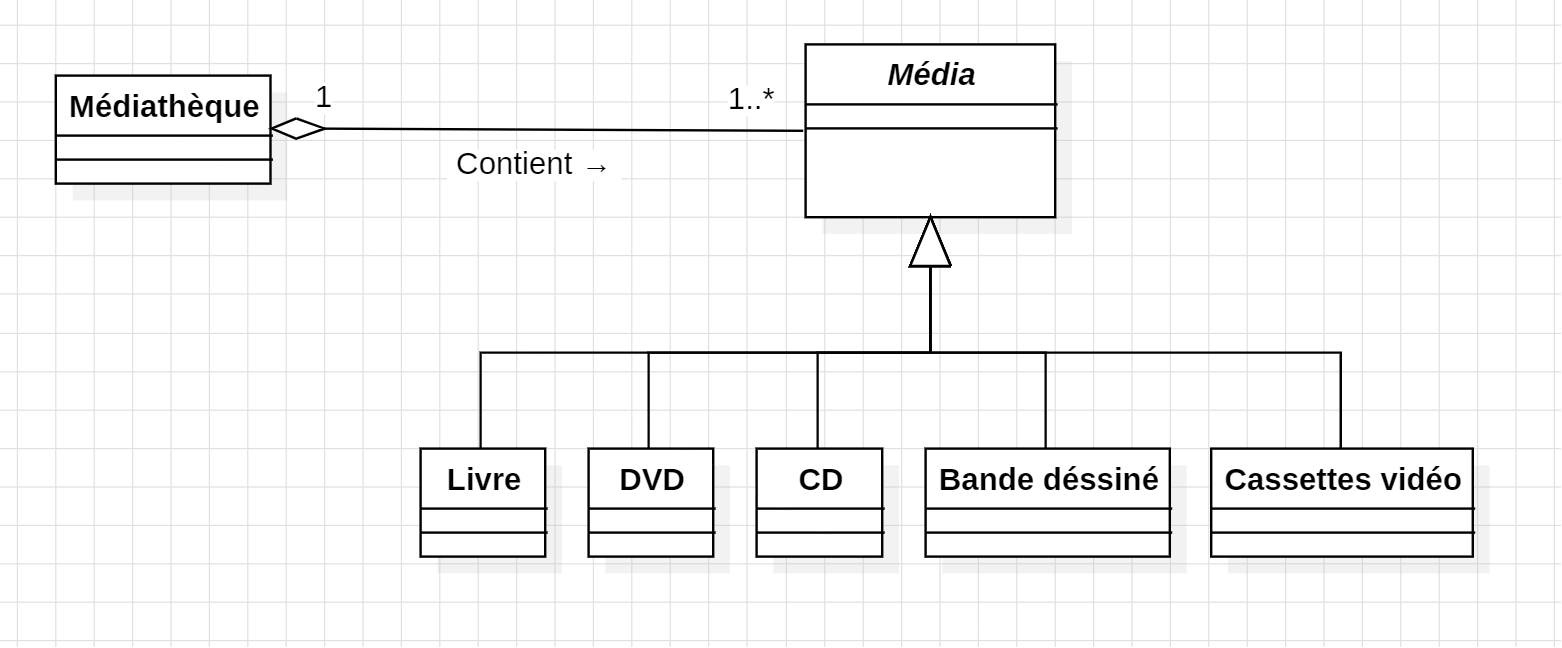
\includegraphics[width=0.6\textheight]{./images/1-1_media.png}
    \caption{Exercice 2.1 : modélisation d'une médiathèque.}
\end{figure}

\subsection{Pays}
\begin{figure}[!htb]
    \centering
    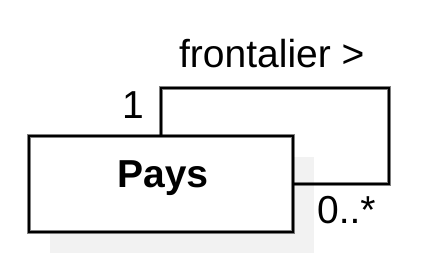
\includegraphics[width=0.16\textheight]{./images/1-2_pays.png}
    \caption{Exercice 1.1 : modélisation de pays frontaliers.}
\end{figure}

\pagebreak
\subsection{Garage}
\begin{figure}[!htb]
    \centering
    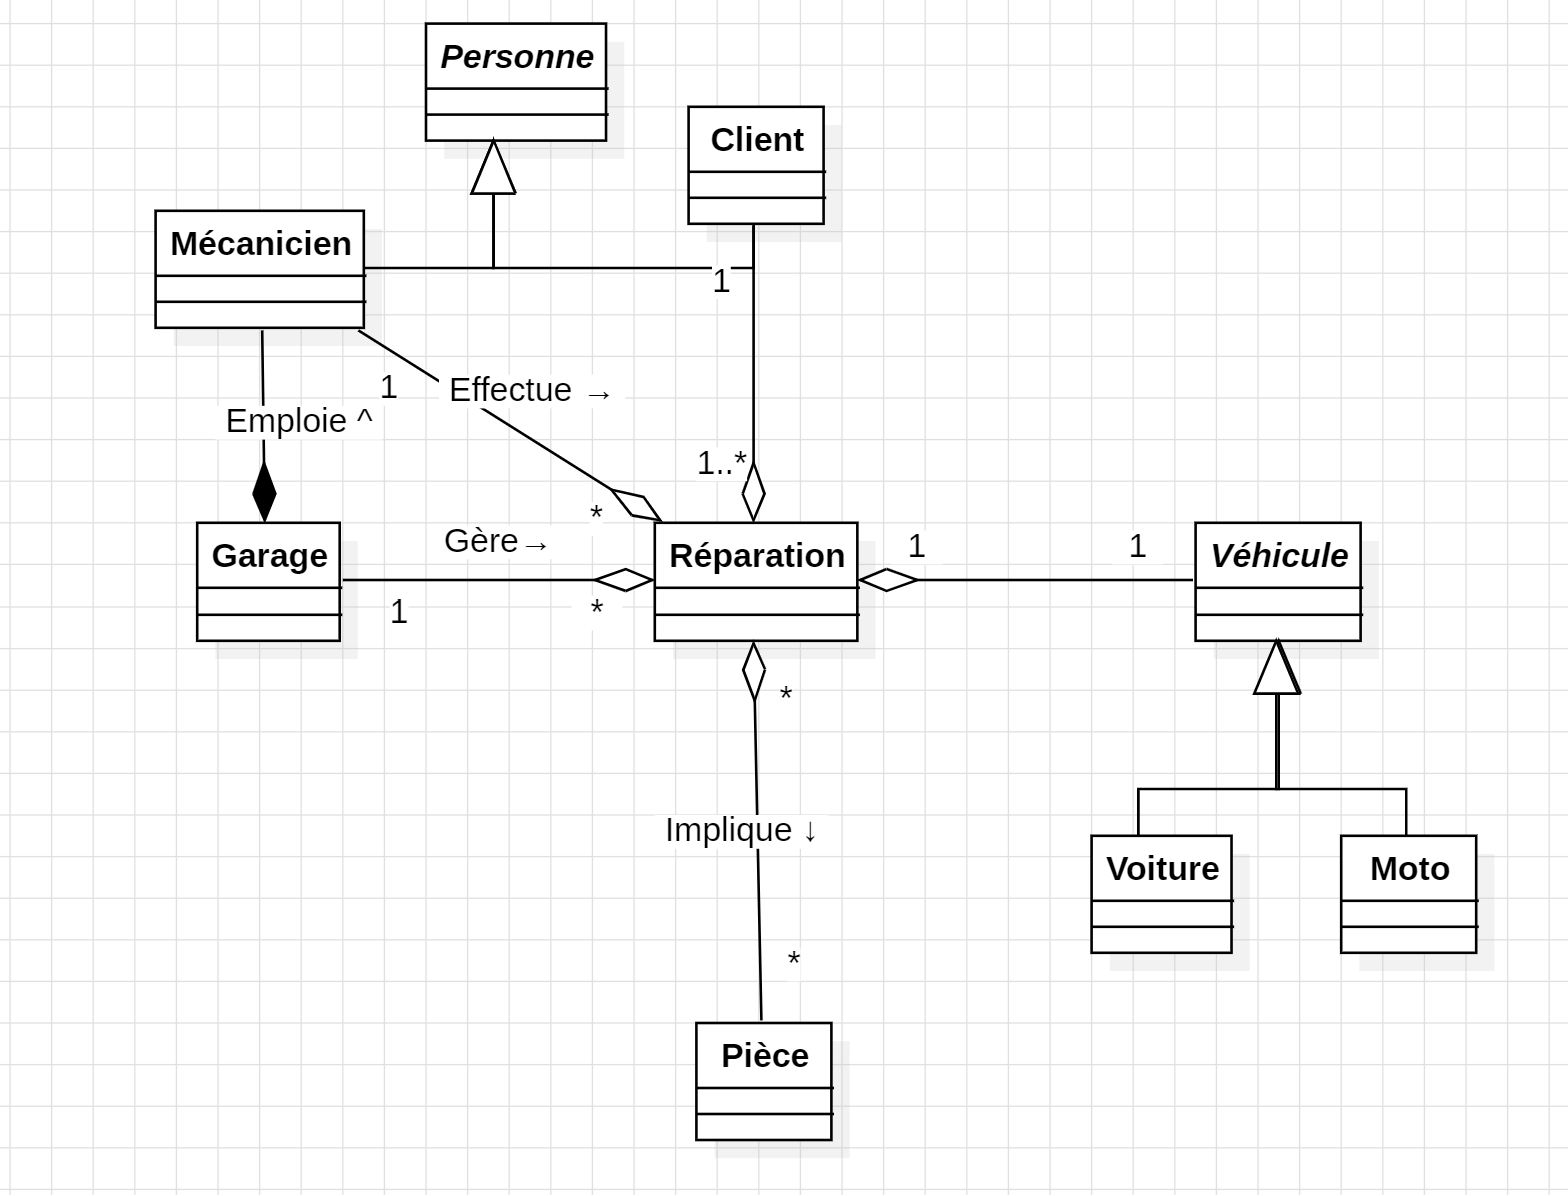
\includegraphics[width=0.5\textheight]{./images/1-3_garage.png}
    \caption{Exercice 1.2 : modélisation d'un garage.}
\end{figure}

\subsection{Paquebot}
\begin{figure}[!htb]
    \centering
    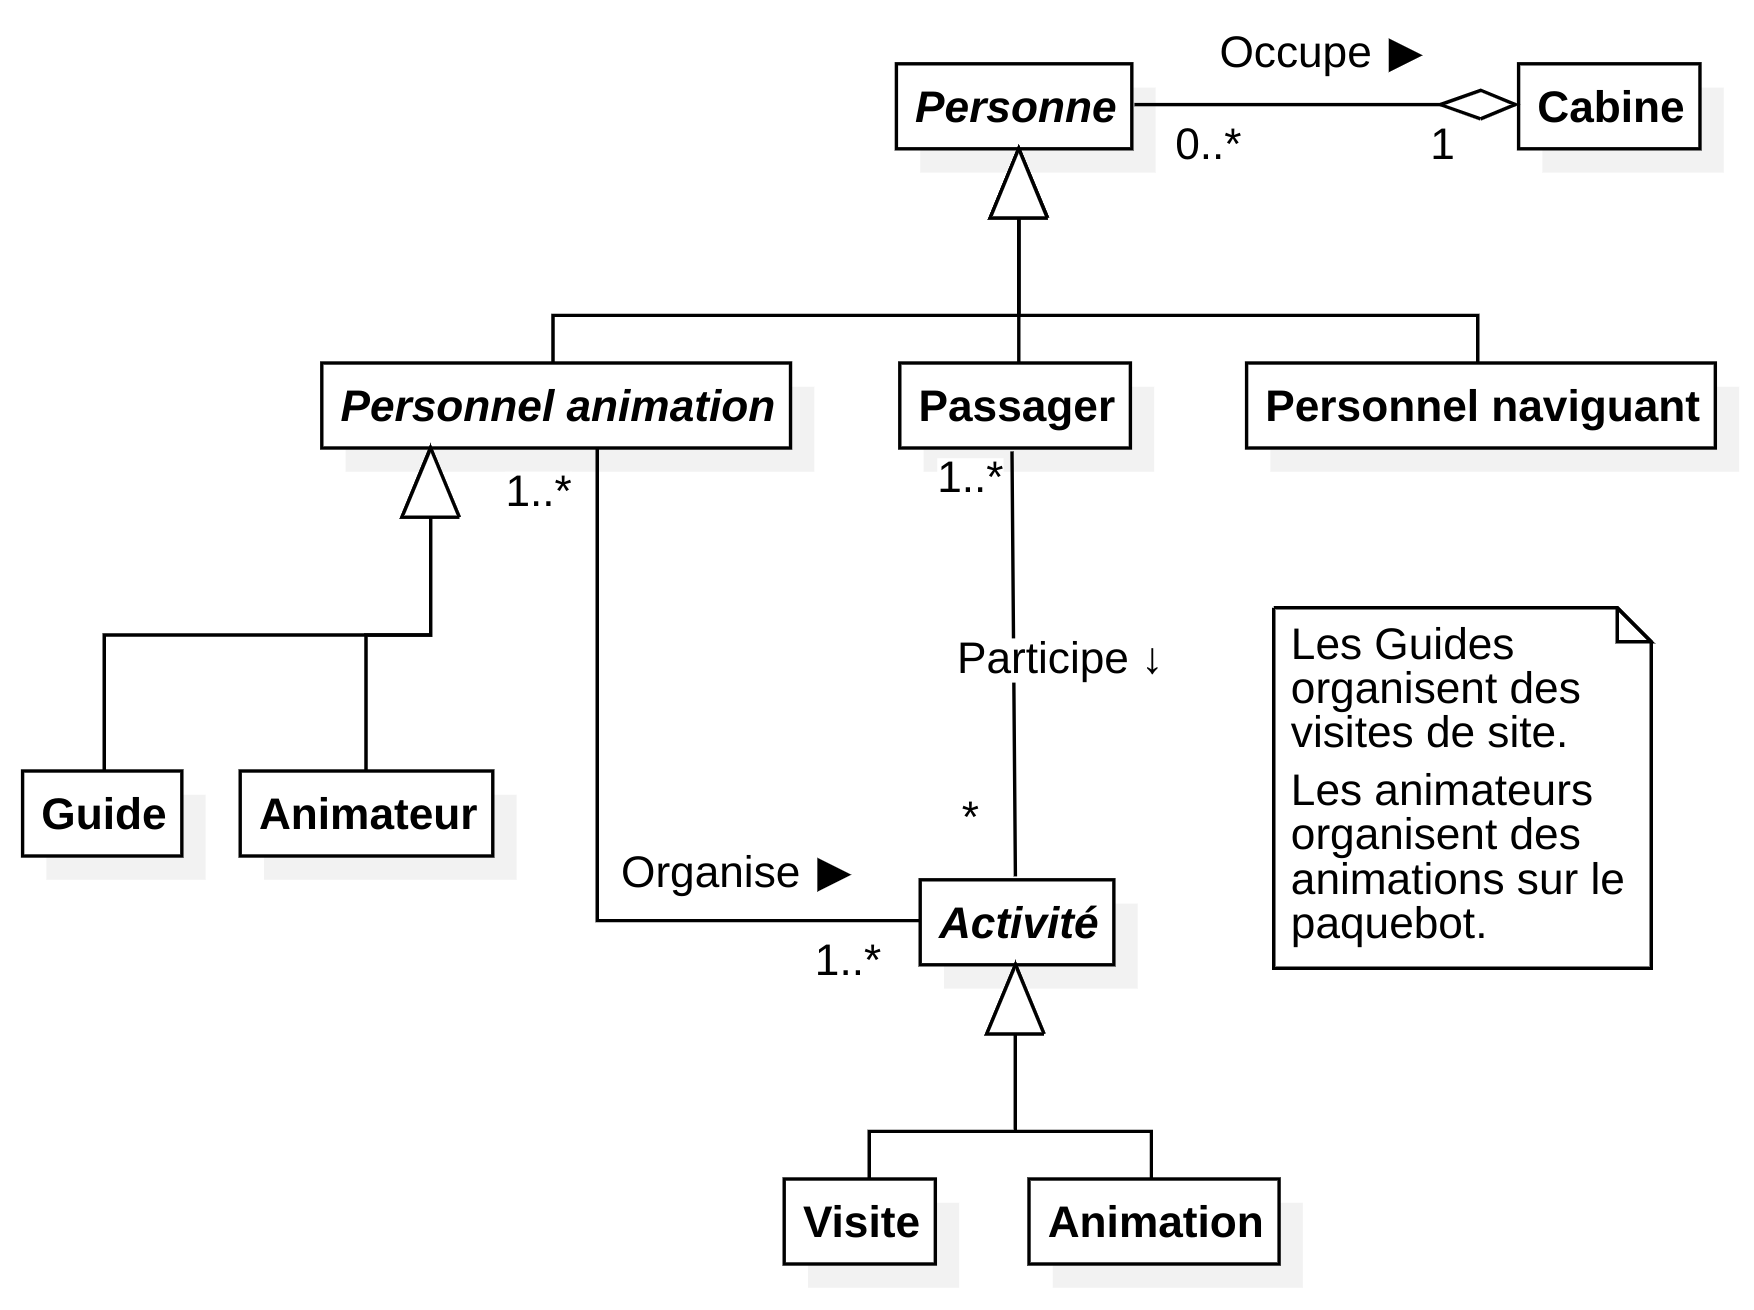
\includegraphics[width=0.5\textheight]{./images/1-4_bateau.png}
    \caption{Exercice 1.3 : modélisation d'un paquebot.}
\end{figure}

\pagebreak
\subsection{Arbre généalogique}
\begin{figure}[!htb]
    \centering
    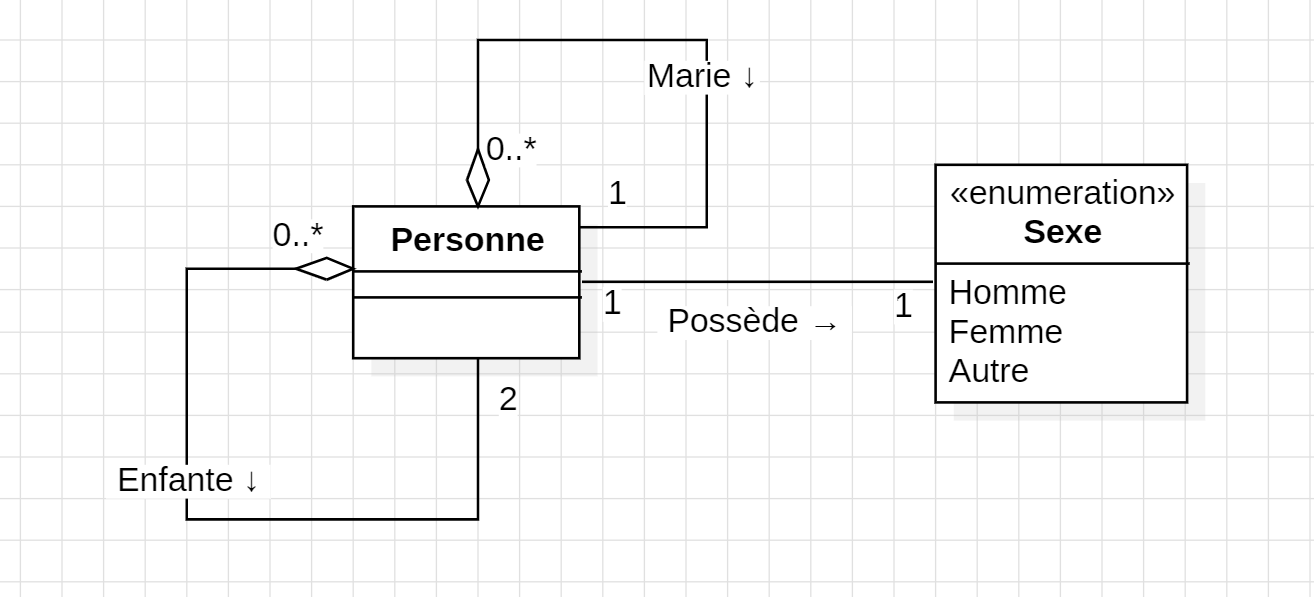
\includegraphics[width=0.5\textheight]{./images/1-5_genealogie.png}
    \caption{Exercice 1.4 : modélisation d'un arbre généalogique.}
\end{figure}

\pagebreak
\section{Modélisations}
\subsection{Éditeur}
\subsubsection{Diagramme de classes}
\begin{figure}[!htb]
    \centering
    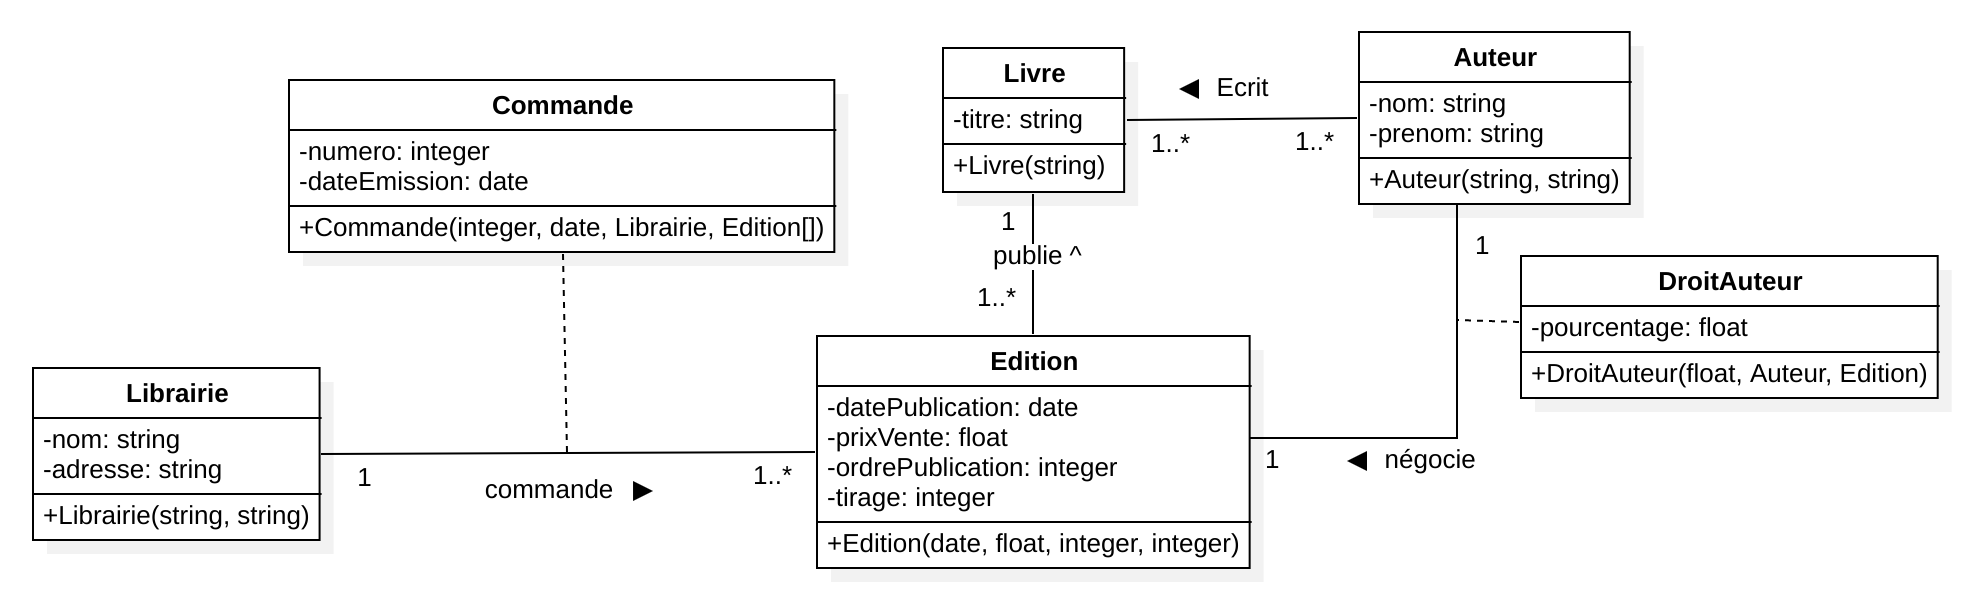
\includegraphics[width=1\textwidth]{./images/2-1_editeur.png}
    \caption{Exercice 2.1 : modélisation d'un éditeur.}
\end{figure}

\subsubsection{Implémentation des associations}
\begin{itemize}
\item Commande : classe particulière Commande
\item Publie : Edition a un attribut référence à Livre et Livre à une liste de références d'Edition
\item Ecrit : Livre a une liste de références d'Auteurs et Auteurs a une liste de références de Livres
\item Négocie : classe particulière DroitAuteur
\end{itemize}

\pagebreak
\subsection{École}
\subsubsection{Diagramme de classes}
\begin{figure}[!htb]
    \centering
    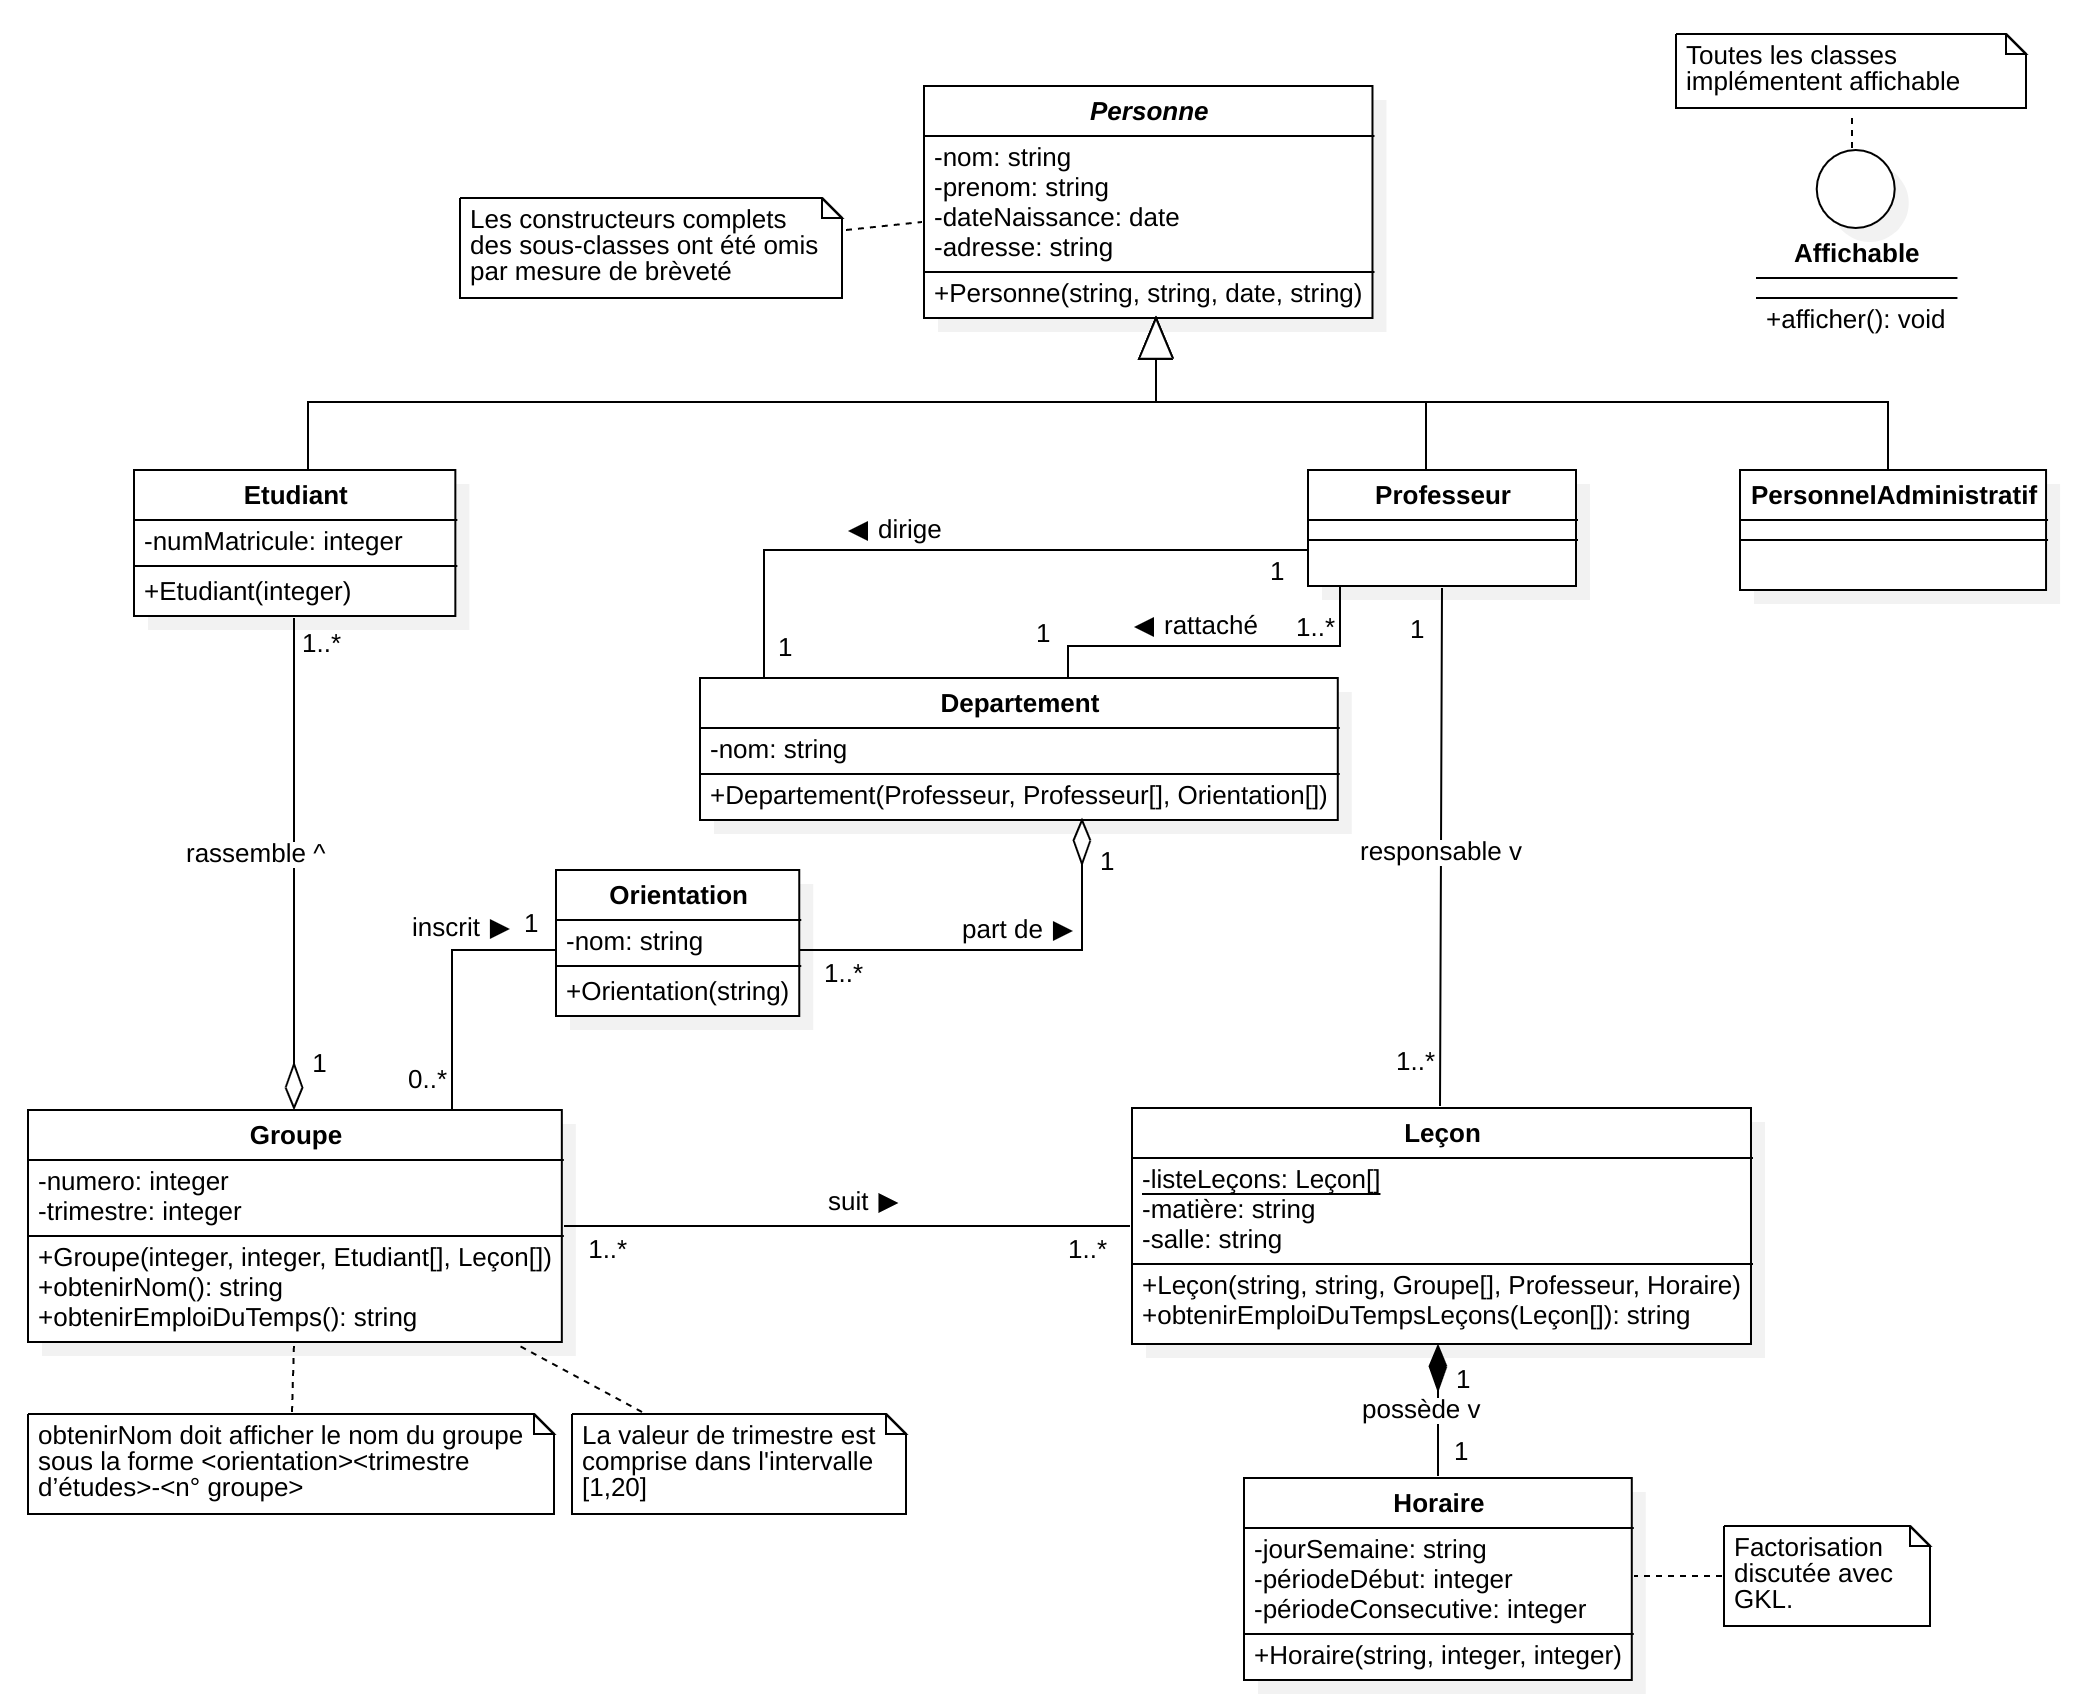
\includegraphics[width=1\textwidth]{./images/2-2_ecole.png}
    \caption{Exercice 2.2 : modélisation d'une école.}
\end{figure}

\subsubsection{Implémentation des associations}
\begin{itemize}
\item Rassemble: Etudiant à un attribut référence de Groupe, Groupe a une liste de référence de Etudiant.
\item Rattaché (Professeur, Departement) : Professeur a un attribut référence de Departement, Departement a une liste de référence de Professeur.
\item Suit : Groupe a une liste de référence de Leçon, Leçon a une liste de référence de Groupe.
\item Part de : Orientation a un attribut référence de Département, Departement a une liste de référence d'Orientation.
\item Responsable : Professeur a un attribut référence de Leçon, Leçon a un attribut référence de Professeur.
\item Dirige : Professeur a un attribut référence de Departement, Departement a un attribut référence de Professeur.
\item Possède : Leçon a un attribut référence de Horaire, Horaire a un attribut référence de Leçon.
\item Inscrit : Orientation a une liste de référence de Groupe, Groupe a un attribut référence de Orientation.
\end{itemize}

\end{document}
